%%%%%%%%%%%%%%%%%%%%%%%%%%%%%%%%%%%%%%%%%
% University/School Laboratory Report
% LaTeX Template
% Version 3.1 (25/3/14)
%
% This template has been downloaded from:
% http://www.LaTeXTemplates.com
%
% Original author:
% Linux and Unix Users Group at Virginia Tech Wiki 
% (https://vtluug.org/wiki/Example_LaTeX_chem_lab_report)
%
% License:
% CC BY-NC-SA 3.0 (http://creativecommons.org/licenses/by-nc-sa/3.0/)
%
%%%%%%%%%%%%%%%%%%%%%%%%%%%%%%%%%%%%%%%%%

%----------------------------------------------------------------------------------------
%	PACKAGES AND DOCUMENT CONFIGURATIONS
%----------------------------------------------------------------------------------------

\documentclass[11pt]{article}

% \usepackage[version=3]{mhchem} % Package for chemical equation typesetting
\usepackage{siunitx} % Provides the \SI{}{} and \si{} command for typesetting SI units
\usepackage{graphicx} % Required for the inclusion of images
\usepackage{xcolor} % 
\usepackage{natbib} % Required to change bibliography style to APA
\usepackage{amsmath} % Required for some math elements 
\usepackage[margin=1in]{geometry}
\newcommand{\tk}{\textcolor{red}}

\setlength\parindent{0pt} % Removes all indentation from paragraphs

% \renewcommand{\labelenumi}{\alph{enumi}.} % Make numbering in the enumerate environment by letter rather than number (e.g. section 6)

%\usepackage{times} % Uncomment to use the Times New Roman font

%----------------------------------------------------------------------------------------
%	DOCUMENT INFORMATION
%----------------------------------------------------------------------------------------

\title{	XSEDE Research allocation TG-CTS150053 \\
	Progress Report 2018\\
	\large{Fully resolved simulations of passive and active particles in fluid flows
}} % Title

\author{Eckart Meiburg} % Author name

\date{\today} % Date for the report

\begin{document}

\maketitle % Insert the title, author and date

\begin{center}
\begin{tabular}{l l}
\multicolumn{2}{l}{UC Santa Barbara, Department of Mechanical Engineering} \\ % 
Office:          & 2351 Engineering II Building \\
Phone:           & (805) 893-5278\\
Email:           & meiburg@engineering.ucsb.edu\\
\\
\multicolumn{2}{l}{Project contributors:} \\ %
Thomas K\"{o}llner    & tk.koellner@mailbox.org\\
Rapha\"{e}l Ouillon    & ouillon@ucsb.edu\\
Rochishnu Chowdhury & rochishnu00@ucsb.edu\\
Bernhard Vowinckel & vowinckel@engineering.ucsb.edu\\
Edward Biegert     & ebiegert@engineering.ucsb.edu\\
\end{tabular}
\end{center}

% If you wish to include an abstract, uncomment the lines below
% \begin{abstract}
% Abstract text
% \end{abstract}

%----------------------------------------------------------------------------------------
%	SECTION 1
%----------------------------------------------------------------------------------------

Our group was awarded 189,188 SUs in node hours by XSEDE for the period of 1/1/2018 -- 12/31/2018 on Stampede2. For the third consecutive year, this allocation has been at the core of our research efforts and progress. It allowed our group to carry out state-of-the-art numerical simulations in the field of computational fluid dynamics to generate high-fidelity data for a variety of aspects related to sediment transport and mixing by active particles in geophysical flows. With XSEDE resources, we conducted studies focusing on three sub-projects: i) Cohesive sediment, investigating the enhanced settling velocity by varying the cohesive forces between particles,  ii) bed erosion by gravity currents, which resolved  the pore-scale interaction of gravity currents propagating over rough, permeable and erodible beds, and iii) swimming induced mixing that studied mixing of stable density stratification by self-propelled organism.
Projects i) and iii) used less resources than originally expected which allowed for a re-evaluation of the scope of project ii). This made it possible to much closer match the experimental apparatus of our collaborators on project ii). All three projects have led to accepted, submitted and pre-submission publications as well as a number of invited seminars and contributions to internation conferences. Below, we provide a brief summary  of the three sub-projects.
\subsection*{Grain-resolving simulations of sediment transport processes}

We have developed a physical and computational model for performing fully coupled, grain-resolved Direct Numerical Simulations of cohesive sediment, based on the Immersed Boundary Method. The model distributes the cohesive forces over a thin shell surrounding each particle, thereby allowing for the spatial and temporal resolution of the cohesive forces during particle-particle interactions. The influence of the cohesive forces is captured by a single dimensionless parameter in the form of a cohesion number, which represents the ratio of cohesive and gravitational forces acting on a particle. Based on this model, we have performed large-scale simulations using XSEDE resources, in order to study the collective behavior of cohesive sediment grains.

As a first step, we have tested and validated the cohesive force model for binary particle interactions in the Drafting-Kissing-Tumbling (DKT) configuration. Cohesive sediment grains can remain attached to each other during the tumbling phase following the initial collision, thereby giving rise to the formation of flocs. The DKT simulations demonstrate that cohesive particle pairs settle in a preferred orientation, with particles of very different sizes preferentially aligning themselves in the vertical direction, so that the smaller particle is drafted in the wake of the larger one. This preferred orientation of cohesive particle pairs is found to remain influential for systems of higher complexity. To this end, we have performed large simulations of 1,261 polydisperse settling particles starting from rest. These simulations reproduce several earlier experimental observations by other authors, such as the accelerated settling of sand and silt particles due to particle bonding, the stratification of cohesive sediment deposits, and the consolidation process of the deposit. They identify three characteristic phases of the polydisperse settling process, viz. (i) initial stir-up phase with limited flocculation; (ii) enhanced settling phase characterized by increased flocculation; and (iii) consolidation phase. The simulations demonstrate that cohesive forces accelerate the overall settling process primarily because smaller grains attach to larger ones and settle in their wakes. For the present cohesion number values, we observe that settling can be accelerated by up to 29\%. We propose physically based parametrization of classical hindered settling functions introduced by earlier authors, in order to account for cohesive forces. An investigation of the energy budget shows that, even though the work of the collision forces is much smaller than that of the hydrodynamic drag forces, it can substantially modify the relevant energy conversion processes.

To date, one manuscript on this topic has been accepted for publication in the Journal of Fluid Mechanics, and a second manuscript is under review with Geophysical Research Letters.
\subsection*{Bed erosion by gravity currents}

During the present allocation period, we laid our main focus on the proposed WP1, which investigates the interaction of a saline gravity current propagating over a bed of large particles that are  not erodible due to their own weight. This was motivated by a fruitful collaboration with the experimental group of Prof. Roger Nokes  from the University of Canterbury, New Zealand that we established during the allocation period. Fig.~\ref{fig:erosion}(a) shows a typical configuration that reproduces the ratio  of the  bed-particle diameter to the flume height used in their experiment. Simulations  altered this ratio as in the experiment where the water level in the flume was changed. These simulation provided novel data on the influence of roughness and permeability on the propagation of gravity currents and  bridge the gap between experiments and simulations. The  results are currently incorporated into a joint publication, were presented at a conference (EFMC 12, Vienna) and will be presented at the 71st Annual Meeting of the APS Division of Fluid Dynamics. For the erodible beds (WP2, WP3), we performed simulation with particles differing in their weight and in the bed configuration (ordered, random).  Fig.~\ref{fig:erosion}(b) shows a density isosurface (green) and neutrally buoyant particles. However our simulation showed that to improve the physical realism of  our simulations, it is inevitable to further reduced the particle diameter, which we propose as a project for the next allocation period.  

\begin{figure}
\centering
\begin{tabular}{cc}
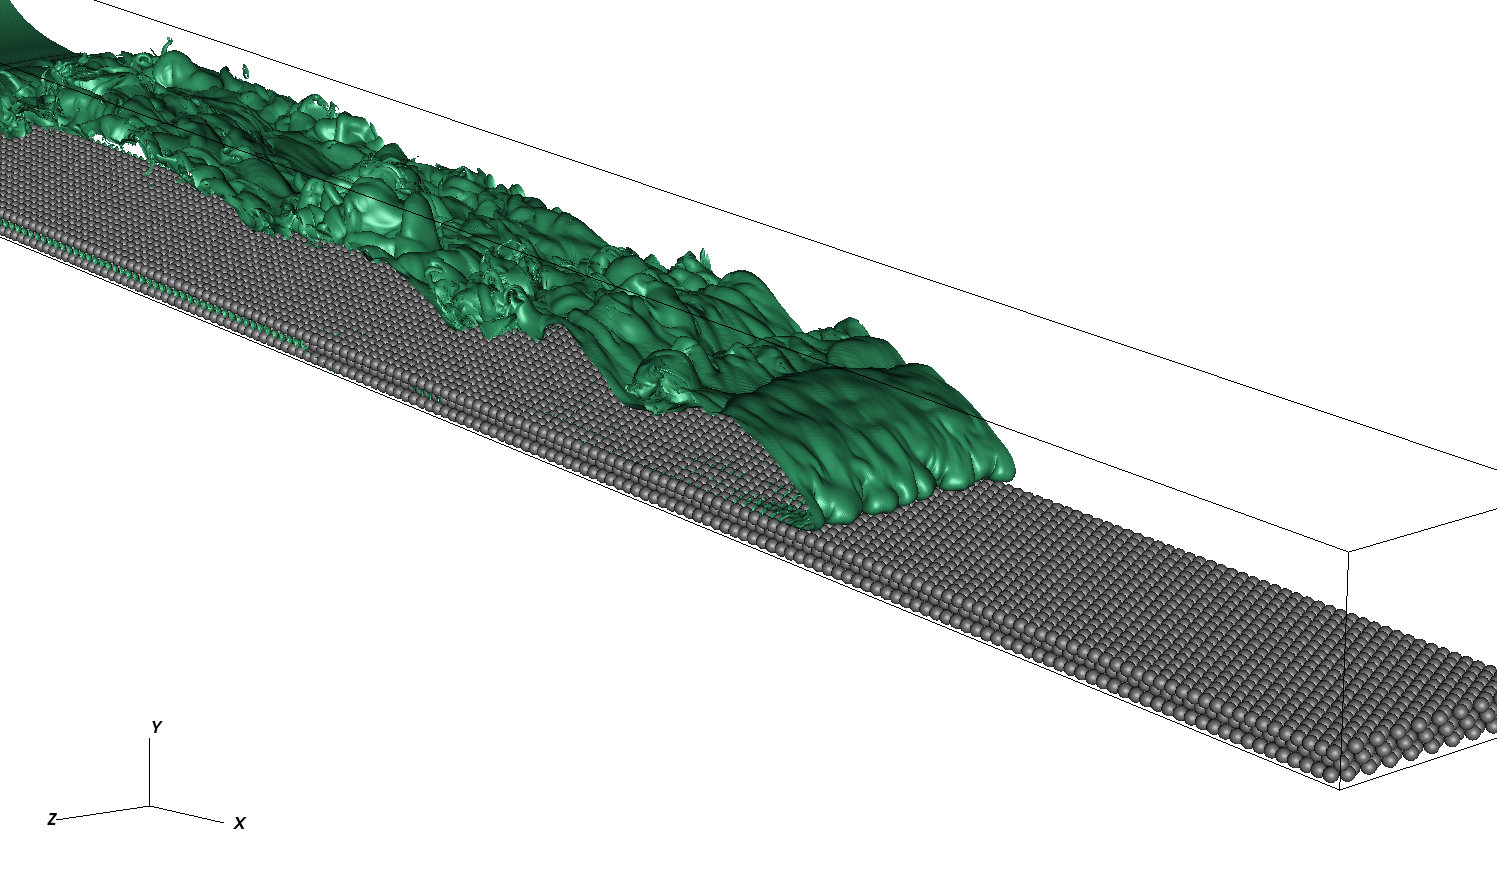
\includegraphics[trim = 30px 180px 30px 50px, clip, width=0.48\textwidth]{figures/iiso0-1_L3h15_t110000.png} &
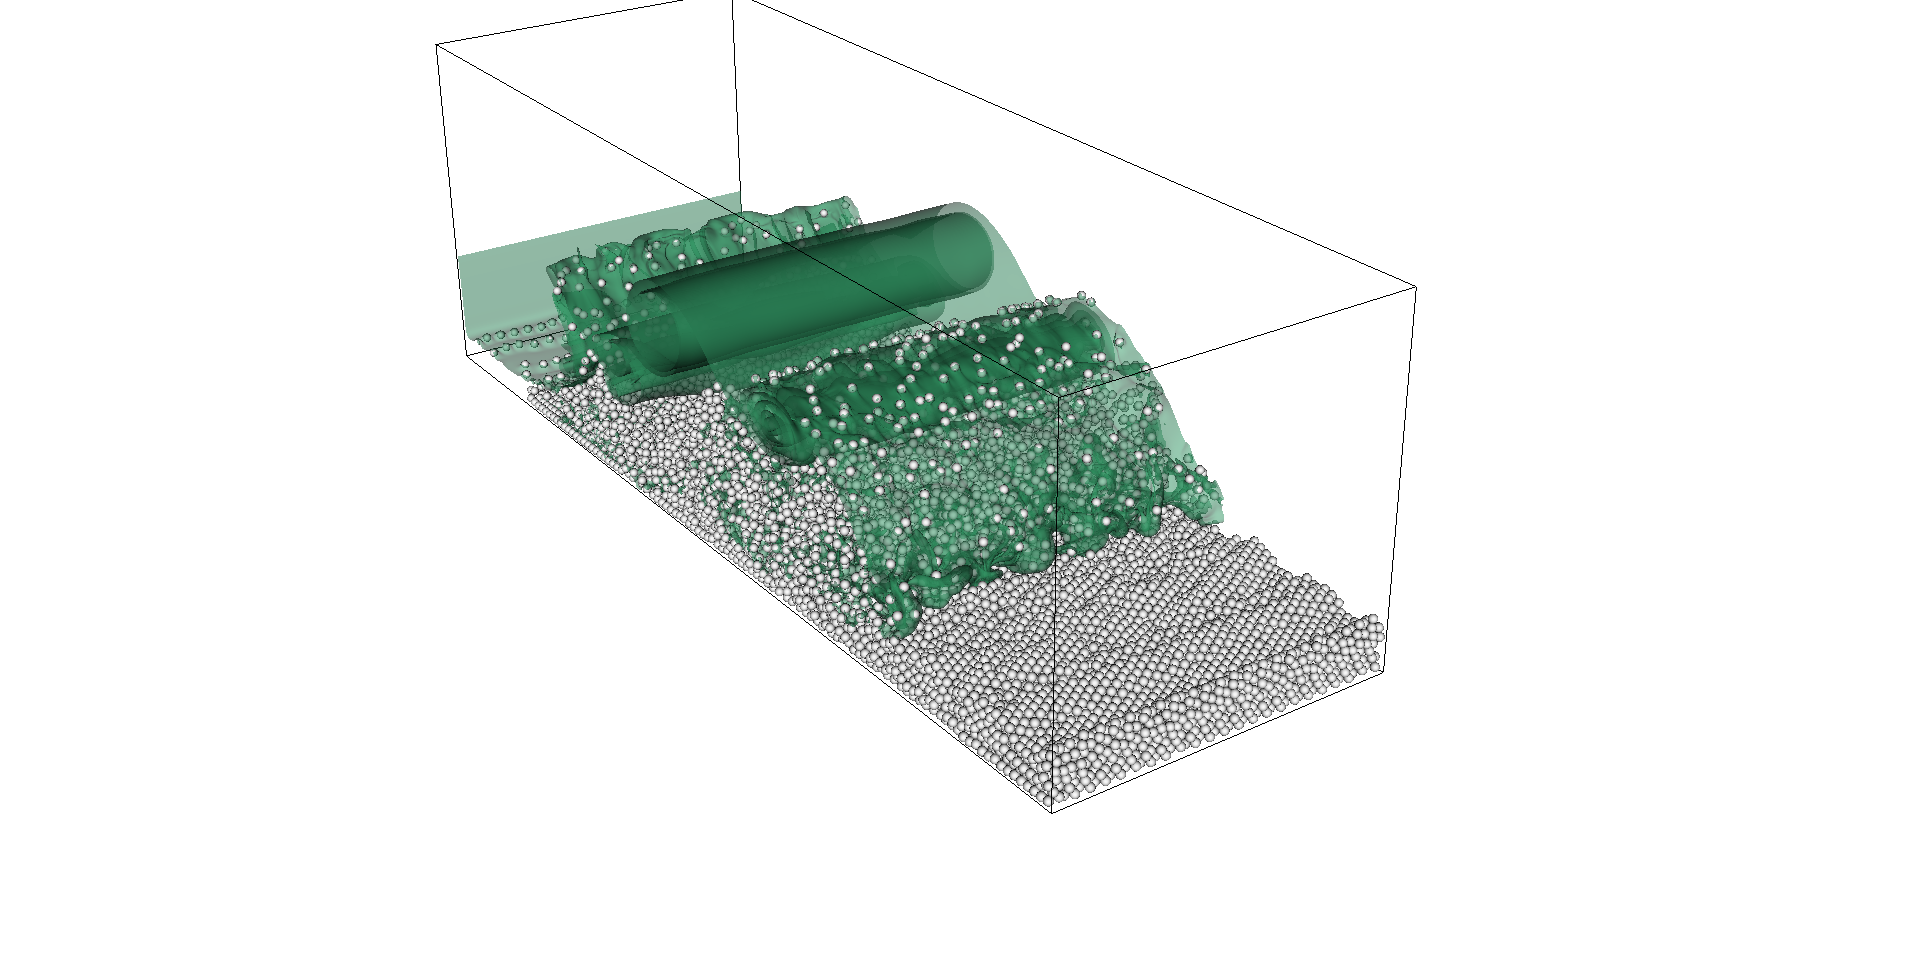
\includegraphics[trim = 250px 180px 350px 50px, clip, width=0.48\textwidth]{figures/E4_0044.png}\\
(a) & (b)
\end{tabular}
\caption{\small \textit{Snapshots of numerical simulation performed within the gravity current project. (a) Density isosurface of gravity current propagating over three-layers of densely packed particles. (b) Density isosurface of a gravity current eroding neutrally buoyant particles. }}
\label{fig:erosion}
\end{figure}


\subsection*{Swimming-induced mixing}
The simulations described in Project 3 WP1-3 of our 2017 proposal were conducted and yielded valuable results. We were able to obtain good agreement between the measured flow-field generated by the swimmers in the numerical simulations and the experimental measurements of our collaborators J. O. Dabiri and I. A. Houghton at Stanford University. The results have been incorporated into a joint manuscript which is now close to submission to \emph{Journal of Fluid Mechanics}. In addition, we improved the numerical handling of the transport of scalars in the presence of swimmers. In particular, the  numerical scheme used to enforce the impermeability of the particles has been further developed and validation simulation were carried out on Stampede 2. An article that describes the developed scheme in conjunction with our swimmer model is in preparation and intended to be submitted to \emph{Computers \& Fluids}.\\

%We would like to mention that two interns in our lab have been trained on Stampede 2. They carried out simulation focusing on sub-problems of the gravity current propagation over permeable bed. Namely,  the porous Rayleigh-Taylor instability that is triggered when dense, saline water overlay a bed soaked in fresh water and the macroscopic modeling of heterogeneous porous media flow. 

In addition to the three main projects detailed in our 2017 proposal, we used a smaller but high-yielding portion of our XSEDE resources on satellite projects. In the frame of our ongoing research on the physics of gravity currents, we conducted high-resolution numerical simulations of gravity currents interacting with internal waves in a two-layer stratification in collaboration with Prof. N. Ouellette and Prof. J. Koseff at Stanford University. We also conducted high-resolution simulations of hyperpycnal flows transitioning to saline turbidity currents. Papers that describe the findings of the two projects have been submitted to \emph{Journal of Fluid Mechanics} and \emph{Geophysical Research Letters} respectively and are currently under review. In the frame of our research on double-diffusive and settling processes, we used XSEDE resources to successfully simulate salt crystallization in double-diffusive fingering convection in the Dead Sea. A paper describing our findings is in preparation in collaboration with Dr. N. Lensky at the Geological Survey of Israel, and is intended to be submitted to \emph{Geophysical Research Letters}.    
% 
%----------------------------------------------------------------------------------------
%	BIBLIOGRAPHY
%----------------------------------------------------------------------------------------

\paragraph*{Peer-reviewed articles (published and submitted, 2018) }  
  \begin{enumerate}
    \item B. Vowinckel, J. Withers, P. Luzzatto-Fegiz, and E. Meiburg, \textit{Settling of cohesive sediment: particle-resolved simulations}, J. Fluid Mech., accepted.
    
    \item E. Biegert, B. Vowinckel, and E. Meiburg, \textit{A collision model for grain-resolving simulations of flows over dense, mobile, polydisperse granular sediment beds}, Journal of Computational Physics 340, 105-127, (2017).

    \item Ouillon, E. Meiburg, N. Ouellette and J. Koseff, \textit{Interaction of a downslope gravity current with an internal wave}, J. Fluid Mech., submitted.
    \item Liang Zhao, Raphael Ouillon, Bernhard Vowinckel, Eckart Meiburg, Benjamin Kneller, Zhiguo He, \textit{Transition of a hyperpycnal flow into a saline turbidity current due to differential diffusivities}, Geophysical Research Letters, submitted.


\end{enumerate}
  
\paragraph*{Invited seminars (2018)}  
  \begin{enumerate}
  

\item T. K\"{o}llner, \textit{Direct numerical simulations of gravity currents propagating
over beds of spherical particles}, Institute of Fluid Dynamics, Helmholtz-Zentrum Dresden-Rossendorf
     

\end{enumerate}
     
  \paragraph*{Conference presentations (2018)}  
  \begin{enumerate}
  
\item T. K\"{o}llner and E. Meiburg, \textit{Numerical modeling of mass and heat transfer for grain-resolving simulations of particle laden flows  }, SoCal Fluids XII, University of Southern California.
  
\item T. K\"{o}llner and E. Meiburg, \textit{Direct numerical simulations of gravity currents propagating over beds of spherical particles},12th European Fluid Mechanics Conference, Vienna, Austria.
\item T. K\"{o}llner, A. Meredith,  C. Cenedese, R. Nokes, and E. Meiburg, \textit{Gravity currents propagating over fixed beds of spherical particles}, 71st Annual Meeting of the APS Division of Fluid Dynamics,  Atlanta, Georgia.
\item R. Ouillon, P. Edel, and E. Meiburg, \textit{Double-diffusive salt-particle systems: The role of settling-driven collective instabilities on the growth of $\gamma$-instabilities}, 71st Annual Meeting of the APS Division of Fluid Dynamics,  Atlanta, Georgia.
  
  \end{enumerate}

\end{document}



%% old part from 2017

\section*{Cohesive Sediment}
\tk{Replace this section with Bernhards work}
Within the current allocation period, we have performed high-resolution, grain-resolving simulations in order to obtain fundamental insight into the dynamics of particulate currents interacting with a sediment bed via erosion and deposition. We have carried out a series of simulations for a conceptually simple  particle-laden Poiseuille flow shown in Figure \ref{fig:poiseuille_flow}, which is similar to the experimental setup of \cite{aussillous2013} and which has been validated in \cite{Biegert2017}. Questions that are currently being investigated are:
\begin{itemize}
\item How does the sediment alter the effective viscosity of the flow? Various authors have come up with rheological models to described particle-laden flows \citep{Morris1999, Boyer2011}, but there is no consensus on a single model to describe all flows.

\item Can the flow be described using a continuum model, such as the one used by \cite{Boyer2011} and \cite{aussillous2013}?  Such a model could be an important predictive tool for sediment fluxes and bedload estimates.

\end{itemize}

To answer the first question, we have been calculating the effective viscosity of the fluid/particle mixture in our simulations.  Figure~\ref{fig:rheology_shear} shows the results from two simulations at different Reynolds numbers, given by $Re = U_b H / \nu$, where $U_b$ is the bulk fluid velocity and $H$ is the entire channel height.  While these simulations show a good collapse of the data for different flow rates, we have been trying to run other cases under a variety of flow conditions in order to establish the universality of the relationship between effective viscosity and volume fraction.

\begin{figure}
\centering
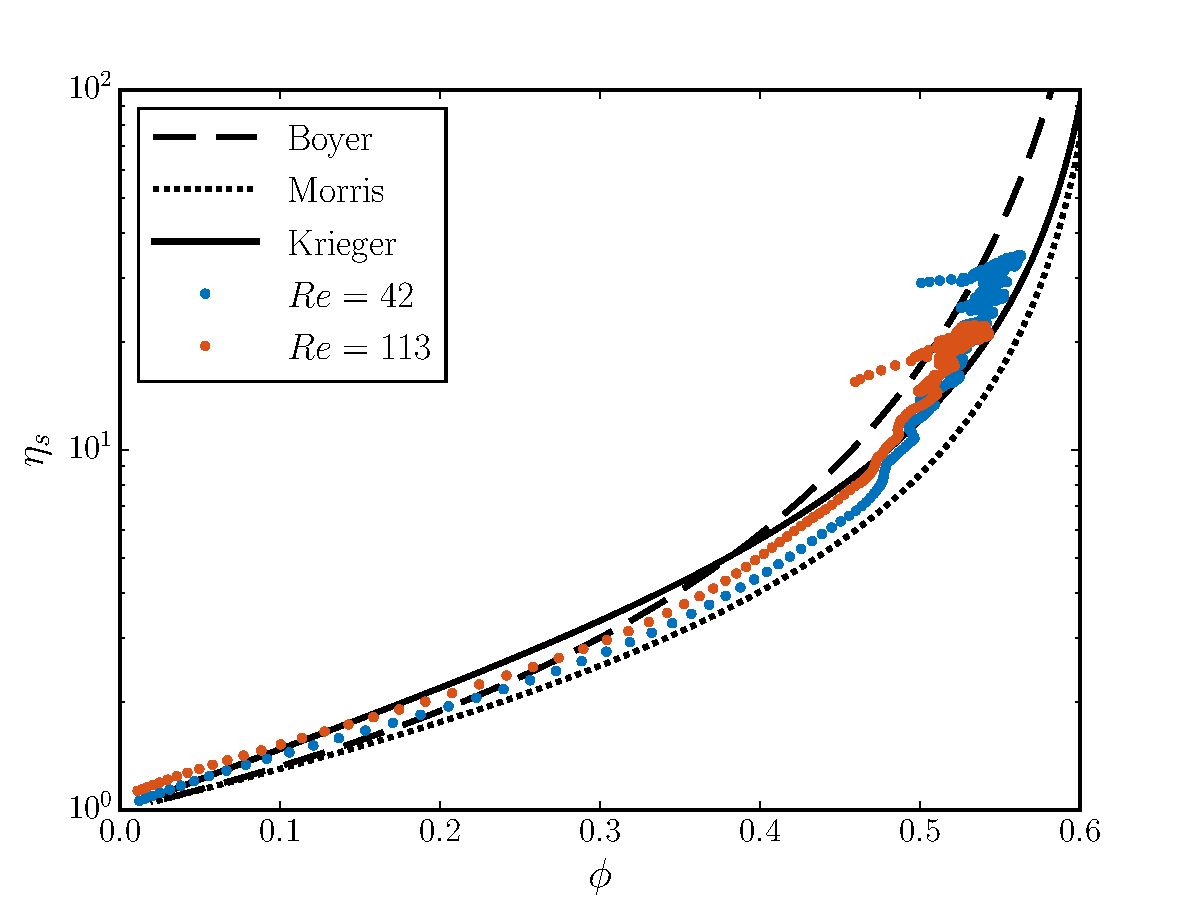
\includegraphics[width=0.65\textwidth]{figures/rheology_shear.pdf}
\caption{\small \textit{ Effective viscosity, $\eta_s$, as a function of the particle volume fraction, $\phi$, for two simulations at different flow rates.  Comparison models are those of \cite{Boyer2011}, \cite{Morris1999}, and \cite{Krieger1959}}}
\label{fig:rheology_shear}
\end{figure}